\section{Docteur Aphra}

\subsection{introduction}
Ce scénario commence dans une cantina pas vraiment accueillante d’Horox III. Les héros aspirent à un peu de repos bien mérité après une mission pour l’alliance qui n’a pas vraiment été une franc succès.

\lettrine{\jedifont{\$}} Ils avaient pour objectif d’identifier l’origine d’un traffic de matrices droïde modifié pour le combat. Malheureusement après deux semaines de recherche et d’intérogatoire infructueux, tout ce qu’ils ont réussit à faire, c’est se prendre une correction par l’un des fameux droïdes modifiés et perdre la trace de leur traffiquant quelque part sur \textbf{Horox III}. 

\lettrine{\jedifont{\#}} Les héros étaient en mission pour l’empire. Ils sont à la recherche d’un individu capable de modifier les matrices de droïde pour en faire des droïdes de combat plutôt performant. Le seigneur Vador se montre très intéressé car il souhaite se monter une armée personelle.

\begin{paperbox}{Objectif}
Les héros sont à la recherche d’un traffiquant de matrices de droïdes.
\end{paperbox}

\subsection{Viens voir le docteur}
\noindent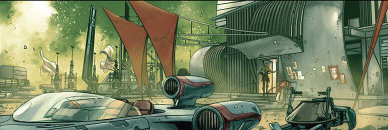
\includegraphics[width=\linewidth]{_img/places/cantina-horox-iii.jpg}
Les voilà donc ruminant leur échec dans un bar quand entre une femme, brune, mince, un bonnet et des lunettes d’aviateur sur la tête. L’horoxien au bar lève la tête et semble, l’espace d’un instant surpris. Puis il se reprend et interpelle violament la femme :

\begin{quotebox}
- \textbf{barman} Aphra ! Tu ne manque pas d’aplomb de te repointer ici ! Les droïdes que tu m’a refilé, c’était de la merde. Ils ont pas tenu 10 minutes !\\
- \textbf{Aphra} En face de ta sale gueule ça m’étonne pas !\\
- \textbf{barman} Attrapez là, on va lui faire sa fête !
\end{quotebox}

Les \nameref{sec:horoxian-barfly}, jusqu’à lors calmes, occupés à leur consommations se lèvent et commencent à pousser les tables. L’ambiance devient très tendu, la bagarre est inévitable. 

Si vos joueurs ont un peu de jujotte, Ils comprennent qu’\nameref{sec:aphra} a quelque chose à voir avec les matrices modifiés qu’ils recherchent, ou qu’au moins elle peut les aider. S’ils ne comprennent pas incitez les à entrer dans la danse avec une bouteille perdu par exemple.

\begin{paperbox}{Baston de bar}
Comptez 2 \nameref{sec:horoxian-barfly} par héros pour que ça soit un peu marrant. Faites aussi en sorte qu’ils n’utilisent pas leurs armes, ça serait trop facile sinon. En gros la mission était fini et ils n’ont pas pris leurs armes avec eux, ou les armes sont interdites dans la cantina.

Au pire, s’ils s’en sortent pas, les \nameref{sec:horoxian-barfly} vont fuir.
\end{paperbox}

\subsection{Docteur \& Queen}

Une fois la baston terminée, les héros interpellent \nameref{sec:aphra}, s’ils n’en font rien, c’est elle qui les accoste.

Soit ils lui demande des infos sur les matrices de droïdes et elle leur prospose un marché, soit, elle leur demande de l’aide pour résoudre un problème en échange d’argent ou d’un artéfacte Jedi. Tout dépend ce qui vais réver vos joueurs.

\nameref{sec:aphra} leur explique alors son problème. Elle possède un artefact contenant la mémoire d’un Jedi mais elle ignore comment l’ouvrir. Par chance, une fois par an, la \nameref{sec:ktath-atn-queen} organise une réception durant laquelle elle accorde un vœux à la personne qui lui apportera la forme de vie organique la plus "étonnante". Et il se trouve que cette réception a justement lieu ce soir, et présenter un spécimen \textit{(montrez le joueur dont le héros présente le plus d’originalité, Jedi, utilisateur de la Force, Wookie, Droïde, \dots)} par les temps qui courent leur assurerait à coup sur l’accès au vœux.

\bigbreak

Une fois la discussion terminée, laissez les héros récupérer leurs armes et faire le plein de munition puis en route pour \textbf{Ktath’Atn.}

\begin{paperbox}{Objectif}
Aider \nameref{sec:aphra} à ouvrir l’artéfacte pour obtenir les renseignements sur le traffic de matrices.
\end{paperbox}